\documentclass[palatino]{epflnotes}

\title{Mathematical modeling of DNA}
\author{Guillermo Julián Moreno}
\date{16/17 - Spring semester}

% Additional packages
\usepackage{siunitx}

% --------------------

\begin{document}
\frontmatter
\pagestyle{plain}
\maketitle

\tableofcontents
\mainmatter
% Content

\chapter{Introduction and overview}

\section{Basics of \sectioncaps{DNA}}

\begin{wrapfigure}[12]{R}{0.4\textwidth}
\centering
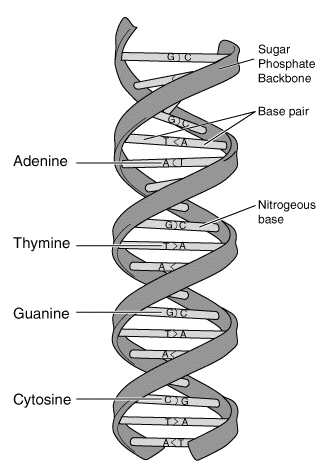
\includegraphics[width = 0.4\textwidth]{img/DNA-structure-and-bases.png}
\caption{Molecular structure of DNA}
\label{fig:DNA}
\end{wrapfigure}

The bases of DNA are denoted by $\mathcal{L} = \set{A,T,C,G}$ with a complementary  rule, where \begin{align*}
\conj{A} &= T &\conj{C} &= G \\
\conj{T} &= A &\conj{G} &= C
\end{align*}

A somewhat interesting fact: the base of the DNA are antiparallel (orientation given by the orientation of the phosphate molecule).

The study of DNA can be separated in its three structures:
\begin{enumerate}
	\item The list of letters $x_i ∈ \mathcal{L} $ for $i = 1, \dotsc, 10^9$ (at least).
	\item The secondary structure is uniform: the double helix.
	\item The tertiary structure relates to the physical properties of the double helix, such as stiffness, which can vary greatly depending on the sequence (up to 25 \%), and its intrinsic shape (the shape of the central line).
\end{enumerate}

Molecular Dynamics simulations of the atoms in DNA and their surrounding medium (water) are considerably expensive, so the focus is in stochastic differential equations for which we can study output probability distribution.

The course-grained model implies simulating not all the atoms but only blocks (sugar, phosphate or whatever is a group for chemists), reducing thus the amount of degrees of freedom.

\section{Course-grained \sectioncaps{DNA} modeling}

We will be interested in models that predict the sequence ground-state structure and flexibility of a sequence. Each configuration space is a vector $\vw ∈ ℝ^N$ and the probability density function $ρ(\vw)$ depends on some constants $Z,β$ and the free energy $U(\vw)$, so that \[ ρ(\vw) = \frac{1}{Z} e^{-βU(\vw)} \]

As the conjugates for each base are clearly defined, we can worry just about the sequence of bases and not the full base pairs. The set of parameters being modeled will by $6n$ intra-basepair and $6(n-1)$ inter-basepair degrees of freedom (see \fref{fig:MovementsDNA}), so a total of $N = 12n - 6$ degrees of freedom for a sequence of $n$ basepairs.

For the cgDNA model, the free energy is approximated as a quadratic form \[ U(\vw)= \frac{1}{2} (\vw - μ) · \mK · (\vw -μ)\] with $μ = μ(S) ∈ ℝ^N$ being the ground state configuration and $\mK = \mK(S) ∈ ℝ^{N×N}$ being the ground-state stiffness, represented by a symmetric and positive-definite matrix.

Of course, the question is how to get those ground states $μ, \mK$ from the sequence $S$ you are studying. The main assumption is that those states are only affected by junction and intra-basepair interaction energies, as shown in \fref{fig:MovementsDNA}, and that the groudn state is the one with minimum energy. During these lectures we will introduce this model and do more things.

\begin{figure}[tbp]
\centering
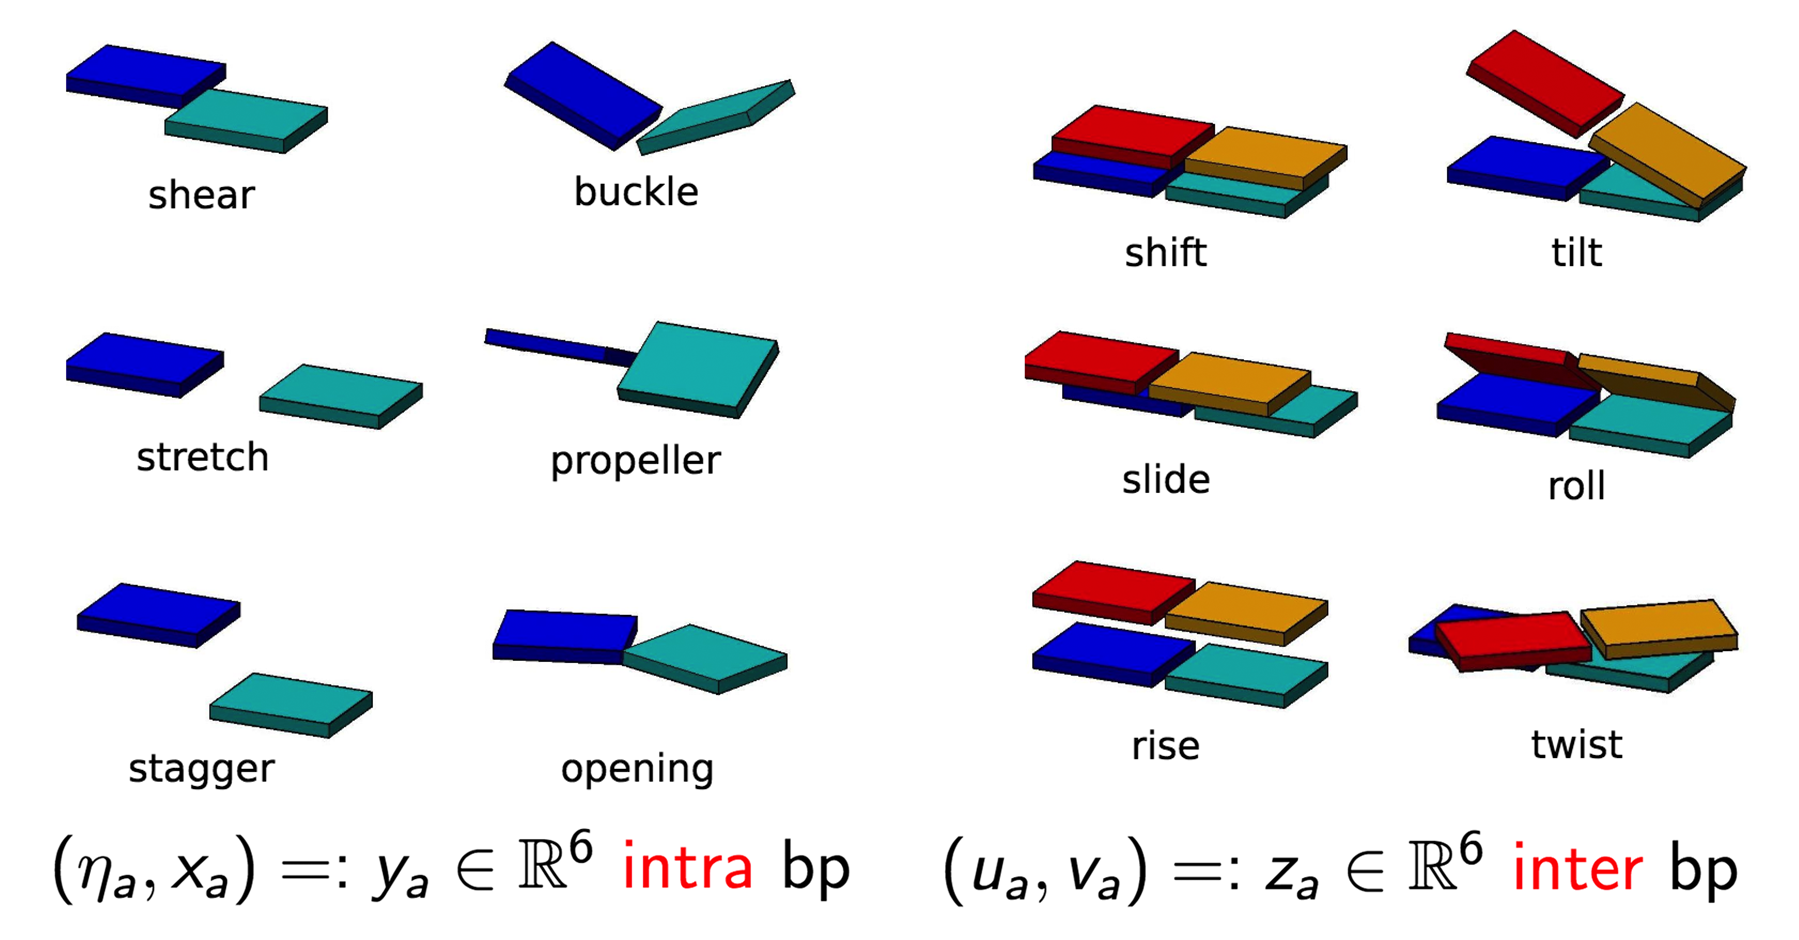
\includegraphics[width=0.8\textwidth]{img/movementsDNA.png}
\caption{Interpair and intrapair interactions}
\label{fig:MovementsDNA}
\end{figure}

\chapter{cgDNA model}

We will consider the coarse-grain model of DNA in which each base on each strand is modeled as an independent rigid body. First, we will define what we mean by an independent rigid body and what mathematical tools do we need to deal with them, and then we will go straight to the modeling.

\section{Rigid body framings: $SE(3)$}

\section{Modeling of \sectioncaps{DNA} sequences}

\subsection{Framing of the base pairs}

\begin{figure}[hbtp]
\centering
\inputtikz{WatsonCrickModel}
\caption{Basic nomenclature in DNA sequences, with $X_i ∈ \set{T,A,C,G}.$}
\label{fig:WatsonCrickStrand}
\end{figure}

We consider a DNA molecule to be identified, as seen in \fref{fig:WatsonCrickStrand}, with a sequence of bases $\set{X_1, \dotsc, X_n}$ along one strand (one side of the helix for us non-biologists), listed in the $5'$ to $3'$ direction (that is, bottom to top). Each base pair is denoted by $(X, \conj{X})_i$, and we will ignore the atoms forming the sugar-phosphate backbones.


For each one of the base pairs we will consider two rigid body motions. One will be referring to the movement between one base and its corresponding one in the other strand, and the other one will model the rigid body motion from one strand to the next one.

\begin{figure}[hbtp]
\centering
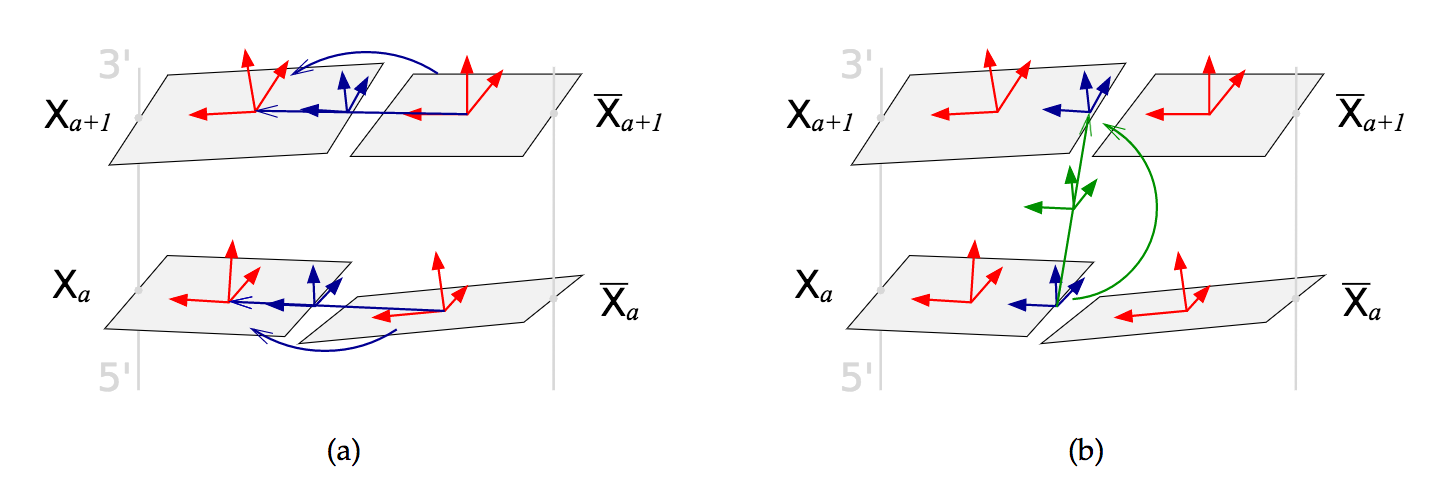
\includegraphics[width=0.8\textwidth]{img/CrickWatson.png}
\caption{A schematic illustration of the base (red), base-pair (blue), and junction (green) frames for an isolated base-pair step.}
\end{figure}

% Missing some week 2 and week 3 material here

What we have then is that, for each level $i$ in the sequence, we have the positions and rotations $R_i^+ ≝ (\mR_i^+, \vr_i^+) ∈ SE(3)$ and $R_i^- ≝ (\mR_i^-, \vr_i^-) ∈ SE(3)$ of both bases (Watson and Crick strands respectively). We are interested in simplifying this and having a parametrization in which we can consider separately between the inter and intra basepair motions.

We will introduce then the position/rotation of the basepair as $R_i ≝ (\mR_i, \vr_i)$ defined as the ``average'' of $R_i^+$ and $R_i^-$. For the rotation that is half the rotation from $\mR_i^+$ to $\mR_i^-$, and for the position that is the midpoint between $\vr_i^+$ and $\vr_i^-$:
\begin{align*}
\mR_i &= \mR_i^- \sqrt{\mQ_i} \\
\vr_i &= \frac{\vr_i^+ + \vr_i^-}{2}
\end{align*} with $\mQ_i = \trans{(\mR_i^-)} \mR_i^+$ the rotation between bases.

In a similar way we can write the displacement between pairs based on the junction frame, defined as \begin{align*}
\mJ_i &= \mR_i \sqrt{\mP_i} \\
\vj_i &= \frac{\vr_i + \vr_{i+1}}{2}
\end{align*} with $\mP_i = \trans{\mR_i} \mR_{i+1}$ being the rotation between base-pair frames.

We can keep on simplifying further: we can get rid of global rotations and translation of the full DNA sequence if we consider not a series of frames and positions but a series of movements and rotations to get from one basepair to another instead.

This leads us to define a set of DNA coordinates starting from an initial assumed configuration $R_1 = (\mop{Id}, \vec{0})$, the intra-pair rigid body motions $Q_i ≝ (\mQ_i, \vq_i)$ and the inter-pair ones $P_i ≝ (\mP_i, \vp_i)$. These allow the calculation of each base position and frame by a recursion relation:
\begin{align*}
\begin{pmatrix} \mR_{i+1} & \vr_{i+1} \\ 0 & 1 \end{pmatrix} &=
	\begin{pmatrix} \mR_i & \vr_i \\ 0 & 1 \end{pmatrix}
	\begin{pmatrix} \mP_i & \sqrt{\mP_i} \vp_i \\ 0 & 1 \end{pmatrix} \\
\begin{pmatrix} \mR_i^+ & \vr_i^+ \\ 0 & 1 \end{pmatrix} &=
	\begin{pmatrix} \mR_i^{-} & \vr_i^- \\ 0 & 1 \end{pmatrix}
	\begin{pmatrix} \mQ_i & \sqrt{\mQ_i} \vq_i \\ 0 & 1 \end{pmatrix}
\end{align*}

The displacements $\vp_i$ and $\vq_i$ can be simply calculated from that relation of recurrence as \begin{align*}
\vp_i &= \trans{\sqrt{\mP_i}} \trans{\mR_i} (\vr_{i+1} - \vr_{i}) = \trans{\mJ} \underbracket{(\vr_{i+1} - \vr_{i})}_{Δ\vr_i} \\
\vq_i &= \sqrt{\trans{\mQ_i}} \trans{(\mR_i^-)} (\vr_i^+ - \vr_i^-) = \mR_i \underbracket{(\vr_i^+ - \vr_i^-)}_{δ\vr_i}
\end{align*}

That is, $\vp_i$ and $\vq_i$ are, respectively, the inter-pair and intra-pair displacements $Δ\vr_i$ and $δ\vr_i$ in the corresponding frames $\mJ_i$ and $\mR_i$. This definition will also be helpful if at some point in the future we want to ``reverse'' the sequences, as we are setting reference frames that will not depend on the direction we traverse the sequence in.

We can improve this a little bit more. Both $\mQ_i$ and $\mP_i$ are in $SO(3)$, that is, we have 9 entries each but there are only 3 independent parameters for each rotation (the ones described in \fref{fig:MovementsDNA}).

So, we need to get to a minimal set of coordinates by introducing the Cayley transform. Provided that neither $\mP_i$ or $\mQ_i$ are close to rotations by π, there exists an unique mapping \begin{align*}
\appl{\cayley}{SO(3) & }{ℝ^3} \\
\mP_i &\longmapsto \vu_i \\
\mQ_i &\longmapsto \veta_i
\end{align*}

The question is, however, in which frame are the components of $\vu_i$. The available optionsare $\mR_i, \mJ_i$ or $\mR_{i+1}$. Similarly, we need to know in which frame are the components of $\veta_i$, as we can have $\mR_i^-$ or $\mR_i$ or $\mR_i^+$.

A nice property of Cayley vector is that it has the same coordinates for all the frames along the rotation, so the answer is that the components of $\vu_i$ are the same in $\mR_i, \mJ_i$ and $\mR_{i+1}$ as it represents the rotation from $\mR_i$ to $\mR_{i+1}$ with $\mJ_i$ being the rotation at the midpoint. The same applies to $\veta_i$.

Finally, we can explain the cgDNA model configuration coordinates. This has, for a $N$ base pair ligomer, a vector $\vw ∈ ℝ^{12N - 6}$ given by $\vw = (\vy_1, \vz_1, \dotsc, \vz_{N-1}, \vy_N)$ where $\vz_i ∈ ℝ^6$ are the inter pair rotations and translations and $\vy_i ∈ ℝ^6$ are the intra pair rotations and translations with the rotations as a Cayley vector. We will sometimes be also interested in vectors $\vx_i = \left(\vy_i, \vz_i, \vy_{i+1}\right) ∈ ℝ^{18}$ for modeling the overlapping of the junctions.

\subsubsection{Inversion of sequences}

We briefly consider here the transformation rule for inversion of a sequence. We will prove later in detail, but if $\vw$ are the coordinates for a specific configuration of the DNA fragment for one choice of the Watson strand then the coordinates $\bar{\vw}$ for the configuration in the reverse sense are $\bar{\vw} = \mE_{2N - 1} \vw$ where \[ \mE_{2N-1} = \begin{pmatrix} 0 & \cdots & \mE \\ \vdots &\iddots & \vdots \\ \mE & \cdots & 0 \end{pmatrix} \] with $\mE ∈ ℝ^{6×6}$ just $-1, +1, +1, -1, +1, +1$ on the leading diagonal.

\subsection{Energy of the DNA sequence configuration}
\label{sec:EnergyDNASequence}

The cgDNA model predicts a probability density function $ρ(\vw; S, P)$ for each configuration $\vw$, depending on the sequence $S$ and the parameter set $P$. For convenience, $S$ and $P$ may be suppressed anywhere in notation.

The assumption is that the PDF is going to be related to an energy distribution, with lower energy states being more probable. Thus, the formula will be something like \[ ρ(\vw; S, P) = \frac{1}{Z} e^{- U(\vw; S, P)} \] where $Z$ is the normalizing constant and $U$ will be quadratic polynomial in $\vw$.

In order to derive the expression for the energy, we assume that the energy of a DNA configuration depends on the energy between bases in a pair and on the cross-junction interaction energies. We assume that all those interactions are quadratic and have minimum-energy states $\hat{\vy}_i$ and $\hat{\vx}_j$ so the energy takes on a form like this: \( \label{eq:ExplicitEnergy} 2U(\vw) = \sum_{i = 1}^N (\vy_i - \hat{\vy}_i) · \mK_{i}^\text{BP} · (\vy_i - \hat{\vy}_i) + \sum_{j=1}^{N-1} (\vx_j - \hat{\vx}_j) \mK^\text{J}_j (\vx_j - \hat{\vx}_j)\) which represent respectively the sum of something over basepairs and sum over junctions, and where where $\vx_j = (\vy_j, \vz_i, \vy_{i+1})$ as defined previously. Also $\mK_i^\text{BP} ∈ ℝ^{6×6}$ and $\mK_{j}^\text{J} ∈ ℝ^{18 × 18}$ are symmetric.

It can be shown that this expression is simplifiable to a single quadratic form if we get rid of constant terms. This expression is
\( \label{eq:SingleQuadraticEnergy} U(\vw) = \frac{1}{2} (\vw - \vmu(S)) · \mK(S) · (\vw - \vmu(S)) \) where $\mK(S) ∈ ℝ^{(12N - 6) × (12N - 6)}$ is a symmetric and positive-definite matrix. Also, $\vmu(S) ∈ ℝ^{12N-6}$ will be the ground-state vector.

An interesting thing about this expression is that, while we have built a model based on local interactions, the ``competition'' between ground states $\hat{\vy}_i$ and $\hat{\vx}_i$ for each of the different energies will imply non-local sequence dependence\footnote{One can show it doing some computations and linear algebra. But it's not interesting.}.

Both the energy matrix $\mK$ and the ground state will have a dependence on both the sequence $S$ and the parameter set $\mathcal{P}$. For now we will not define the parameter set as it is \textit{a lot} of work\footnote{Probably weeks 8-13 of the course.} and we will just assume it given as it changes only rarely.

\subsubsection{Sequence dependence}

We need to detail from there are the matrices and ground states coming from. Given a sequence of bases $S = \set{x_1, x_2, \dotsc, x_N}$, we will first select the stiffness matrix $i$ as $\mK_i^\text{BP} = \mK^{x_i}$, where $\mK^A, \mK^T, \mK^C, \mK^G ∈ \mathcal{P}$ are given matrices in the parameter set.

That is, we make the assumption that $\mK_i^\text{BP}$ depends only on the composition of the basepair $i$ (that is, the bases) and not on the order of that basepair in the sequence. Similarly assume that $\hat{\vy}_i = \hat{\vy}_{x_i}$ depends only on the bases and not on the position.

The matrices for the junctions are obtained with an analogous assumption: they only depend on the composition of the bases of the junction, so that $\mK_j^\text{J} = \mK^{x_j, x_j+1}$ with $\mK^\text{AA}, \mK^\text{AT}, \dotsc, \mK^{\text{CC}}, \mK^\text{CG} ∈ \mathcal{P}$. We will force these matrices to be symmetric and as we did previously, force $\hat{\vx}_i$ to depend only on the bases and not on their positions.

It is important to see that, for now, we have introduced only local dependence of parameters on the sequence.

Another interesting question is to see why have we chosen quadratic forms for energy. The answer is that it seems to fit with experimental data. It is, however, a big approximation.

We will assess the validity of these assumptions later in the course. For example, there are complications in the first and last junctions and base-pairs, and this is a current research topic.

\subsubsection{Connection between explicit equation and single quadratic form and conditions on stiffness matrices}

We are going to explore a little bit more the connection between the explicit equation of energy \eqref{eq:ExplicitEnergy} and the single quadratic form \eqref{eq:SingleQuadraticEnergy}. By doing a bit of linear algebra, we can show that \[ (\vx - \va) \mA (\vx - \va) + (\vx - \vb) \mB (\vx - \vb) = (\vx - \vc) \mC (\vx - \vc) + \text{constant} \] where $\mC = \mA + \mB$ and $\vc = \inv{\mC}(\mA \va + \mB \vb)$. We can use this to express the sums of \eqref{eq:ExplicitEnergy} in a single quadratic form, getting rid of the constant which is not relevant for energy-minimization purposes.

\begin{figure}[hbtp]
\centering
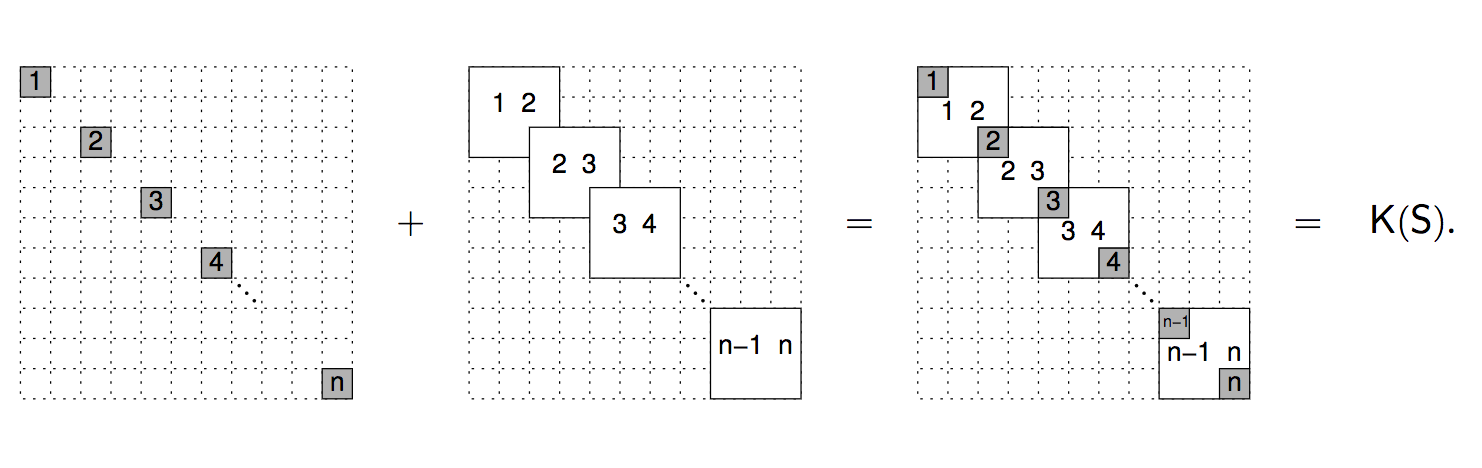
\includegraphics[width=\textwidth]{img/StiffnessBuilding.png}
\caption{Gray matrices represent basepair matrices, white represent junction matrices and the numbers define the index of the corresponding basepairs.}
\label{fig:StiffnessBuilding}
\end{figure}

In our case, for the summation of two matrices of different dimension we will have to ``pad'' with zeros and build the corresponding matrix, as can be seen in \fref{fig:StiffnessBuilding}.

Based on this formulation, we can infer some properties of the resulting stiffness matrix $\mK$ that are valid for any sequence. First, as all junction and basepair matrices are symmetric, $\mK$ is symmetric too.

A second property is that $\mK$ is banded. Particularly, the sparsity pattern is overlapping $18 × 18$ blocks. This is \textit{a big assumption} that will play a big part in estimating parameter sets. Physically, this means that the interactions modeled are only corresponding to the nearest neighbors of each base.

Finally, we want to see when is $\mK$ positive definite. Recall that a symmetric matrix is positive-definite if and only if $\trans{\vx}\mA \vx > 0$ for all $\vx ≠ 0$. Assume all the junction and basepair matrices $\mK^α, \mK^{α,β}$ are positive definite ($α,β ∈ \set{C,G,A,T}$). Then, $\mK$ must be positive definite because of its definition as $\trans{\vx} \mK \vx = \sum \vy \mK^α \vy + \sum \vz \mK^{α,β} \vz$.

However, this condition is too strong and can lead to indefinite matrices with eigenvalues too close to zero. A weaker sufficient condition is just to have \begin{align*}
\mK^α + \mK^{α,β} + \frac{1}{2} \mK^β &> 0 \\
\frac{1}{2} \mK^α + \mK^{α,β} +  \frac{1}{2} \mK^β &> 0
\end{align*} which allows us to have negative eigenvalues on $\mK^α$ for some values.

The sum of matrices with different dimensions is done with $\mK^α$ a block in upper left corner and $\mK^β$ in lower right corner (there are $3×3$ blocks of size $\dim \mK^α$ in $\mK^{α,β}$ and I should understand what this is).

In order to prove this, one has to ``expand'' the stiffness matrix so that no overlaps occur, in a way that all the blocks are of the two forms presented above. One can prove that, if $\vx = (x_1, x_2, \dotsc, x_N)$ and $\mC$ is the ``expanded'' matrix form of $\mK$, then $\trans{\vx} \mK \vx = \trans{\vz} \mC \vz$ with $\vz = (x_1, x_2, x_3, x_3, x_4, x_5, x_5, \dotsc)$. So, if $\mC$ is positive definite, $\mK$ is positive definite too.

An interesting issue arising from this is that basepair matrices having negative eigenvalues imply that some pairs do not have minimum ground-states and then may blow apart. Turns out that it is actually something that happens in reality: short DNA polymers ($N < 5$) disintegrate.

\subsubsection{Conditions on shifts $\vec{μ}(S)$ and non-local dependence}

As we explained previously, we assumed that the ground state vectors $\hat{\vy}_i = \hat{\vy}^α$ and $\hat{\vx}_i = \hat{\vy}^{α,β}$ are given in the parameter set and depend only on the bases $α,β ∈ \set{C,G,A,T}$.

Thus, the calculation of $\vec{μ}$ simply implies solving the linear system: \[ \mK \vec{μ} = \sum_{i=1}^N \mK_i^\text{BP} \hat{\vy}_i + \sum_{j=1}^{N-1} \mK_j^\text{J} \hat{\vx}_i \]

A remark is that naked values of $\hat{\vy}^α$ and $\hat{\vx}^{α,β}$ never appear so the parameter set only stores the values of $\vec{σ}^α = \mK^α \hat{\vy}^α$ and $\vec{σ}^{α,β} = \mK^{α,β} \hat{\vx}^{α,β}$. This also works pretty well with the calculations of matrix overlapping, as we can define \[ \vec{σ}(S) = \sum \vec{σ}_i^\text{BP} + \sum \vec{σ}_j^\text{J}\] and \[ \mK \vec{μ} = \vec{σ} \iff \vec{μ} = \inv{\mK} \vec{σ} \] which gives non-local sequence dependence of $\vec{μ}$, as the inverse matrix $\inv{\mK}$ is dense.

\subsubsection{Some extra remarks on the cgDNA model}

Recall that the energy is \( ρ(\vw; S, P) = \frac{1}{Z} e^{ - \frac{1}{2} (\vw - \vmu(S)) · \mK(S) · (\vw - \vmu(S))} \label{eq:EnergyPDF} \) which we can regard as a Gaussian PDF. Despite the fact that we have vectors in specific spaces (specially the Cayley vectors) we will use the usual Lebesgue measure in $ℝ^{12N - 6}$ when we perform integrals, as that will allow us to use the regular formulas for Gaussian functions in multiple dimensions.

We also recall from the last exercise session\footnote{TODO: Actually do these exercises. Week 5 session.} that the PDF of a sequence $S$ defines exactly the PDF of the complementary $\conj{S}$, with \begin{align*}
\conj{\vec{μ}} &= \mE_n \vec{μ} \\
\conj{\mK} &= \mE_n · \mK · \mE_n
\end{align*}

In the specific case of palindromic sequences, we have as expected $\conj{S} = S$ which implies constraints on the cgDNA ground state, namely $\vmu = \mE_n \vmu$ and similarly for $\mK$. These will be considerably important later for parameter estimation.

Yet another unrelated remark is that we need a discussion of the units of entries in $\vmu$ and $\mK$, and we will discuss those later again.

\chapter{cgDNA experiments}

Once we know the model, we can start performing experiments with it. We have as discussed previously a Gaussian probability density function, and we will use it to calculate certain expectations and probabilities. In particular, we will look at two experiments: the first will look at the probability of configurations with two fixed ends, and the second something spaghetti.

These experiments require a minimum of one hundred basepairs, and are thus way beyond the capabilities of molecular dynamics simulations.

For experiments with fewer basepairs such as NMR (Nuclear Magnetic Resonance) and X-Ray crystal structures, the reports are that the shapes are a function of sequences, so those results are used for estimation of parameters for the cgDNA model.

For NMR and X-Ray crystal experiments, the rigid base movements can be observed and the full vector $\vw ∈ ℝ^{12N - 6}$ can be computed. For the two experiments that we will look at below (looping and persistence length), the length of the strand implies that it is impossible to get those intra base-pair parameters and thus we will only see the shapes parametrized by the inter base-pair rigid body motions.

Therefore, we will compute expectations and probabilities on the base pair frames $(\mR_i, \vr_i)$ and we won't need the intra basepair frames (although they will play an important role in the computation later on). Also, those frames $(\mR_i, \vr_i)$ are a complicated, nonlinear function of the inter variables in junctions $1, 2, \dotsc, i - 1$, and even when we have a Gaussian we will not be able to easily compute expectations and probabilities of $(\mR_i, \vr_i)$.

The main advantage, however, is that it is very easy and efficient to sample random numbers with a normal distribution so Monte Carlo techniques will be very well suited for our purposes. Using the cgDNAmc software, based on a sequence and parameters $\set{S, \mathcal{P}}$ we will get a set $\set{\vw^j}_{j = 1}^M$ of $M$ possible positions\footnote{For us, $M \sim 10^6$. With HPC techniques you can get to $10^{14}$.} and then we can approximate moments $\pesc{φ(\vw)}$ as \[ \pesc{φ(\vw)} = \frac{1}{Z} \idotsint\limits_{ℝ^{12N - 6}} φ(\vw) ρ(\vw) \dif \vw \approx \frac{1}{M} \sum_{j=1}^M φ(\vw^j) \]

\section{Persistence length experiments}

As discussed above, for persistence length experiments we will be interested in computing the expectations of two specific functions, pretty common in polymer physics. First,
\(φ_n(\vw) = \mR_1^T (\vr_n - \vr_1) ∈ ℝ^3, \; n = 2, \dotsc, N \label{eq:FloryVector} \)
which is the end to end chord vector in components of the first base pair frame. This is sometimes called the \concept{Flory\IS vector}. It is important to fix the coordinates to avoid having a zero average because of symmetry.

The second choice of function to study is \( \label{eq:RotationMatrixPerslength} γ_n(\vw) = \mR_1^T \mR_n ∈ SO(3),\; n = 2, \dotsc, N \) which is the relative rotation of the orientation between the first and the $n$th basepairs.

The point is that given a configuration $\vw$ in the internal cgDNA coordinates, we can compute both $φ_n$ and $γ_n$ as a function of $\vw$ with a horrible but explicit function.

To define correctly all those transformations, we define $\mX_n = (\mR_n, \vr_n) ∈ SO(3)$ as the usual matrix representation. We also have the recursion \[ \mX_n = \mX_{n-1} \left(\mQ_{n-1}, \vq_{n-1}\right) \] where $(\mQ_{n-1}$, $\vq_{n-1})$ is the $n-1$ junction rigid body motion. We also know that $\mQ_{n-1} = \mop{Cayley}(\vu_{n-1})$ so that we can reconstruct everything.

What we will do is to plot $\log γ_n$ and $φ_n$ with respect to $n$ and what we will observe is that $\log γ_n$ is close to linear but with different slopes for each sequence, and that $φ_n$ tends to a single point for different sequences.

We don't actually know how to prove that behavior with the cgDNA model. However, we will be able to do it for simpler rigid base-pairs with nearest-neighbor rigid base interactions and an uniform chain.

A simple proof is the following. We have the recursion $\mX_n = \mX_{n-1} \mA_{n-1}$ with $\mA_{n-1} ≝ (\mQ_{n-1}, \vq_{n-1}) ∈ SE(3)$, so that $\mX_n = \mX_1 \mA_1 \dotsb \mA_{n-1}$ so that \[ \inv{\mX_{1}} \mX_n = \prod_{k = 1}^{n - 1} \mA_k\]

We also know that $\inv{\mX_1} = (\trans{\mR_1}, - \trans{\mR_1}\vr_1)$ and then \[ \prod_{k = 1}^{n - 1} \mA_k = ( \trans{\mR_1} \mR_n, \trans{\mR_1}(\vr_n - \vr_1))\] which are , by no accident, the choices we made for $φ_n$ and $γ_n$. This implies that the expectation \[ \pesc{\mX_1^{-1} \mX_n} = \pesc{\prod_{k=1}^{n-1} \mA_k} = \prod_{k=1}^{n-1} \pesc{\mA_k} = \left(\pesc{\mQ_k}, \pesc{\vq_k}\right)  \]
assuming nearest-neighbor rigid base pair functions (not true for cgDNA). Thus, if the chain is uniform\footnote{?¿?¿?¿} we have $(\pesc{\mQ}, \pesc{\vq}) ≝ (\mY, \vy)$ with $\norm{\mY} < 1$ and then \[ \pesc{\inv{\mX_1} \mX_n} = (\mY, \vy)^{n-1}= (\mY^{n-1}, (I + \mY + \mY^2 + \dotsb + \mY^{n-1})\vy))\]  which is why it goes down exponentially, with $\mY^{n-1} \to 0$. Additionally, we have that $(I + \mY + \mY^2 + \dotsb + \mY^{n-1})\vy) \to (I - Y)^{-1} \vy$.

Despite having made assumptions that are not valid for the cgDNA model, these results will be valid for those simulations.

We are going to tle bit on the specifics of all of this. We will start by the proof that $\pesc{\mR_1^T \mR_n} = \pesc{\cos θ_{1,n}} \to 0$.

Assume that the matrix $A_n = (\mQ(\vu), \vq)$ are i.i.d junctions displacements, with $\vq$ constant and $\mQ(\vu)$ given as the matrix associated to the Cayley vector $\vu ∈ ℝ^3$ as \[ \mQ(\vu) = \frac{1 - \norm{\vu}^2}{1 + \norm{\vu}^2} I + \frac{1}{1 + \norm{\vu}^2} \vu^× + \frac{2}{1 + \norm{u}^2} \vu \otimes \vu \]

We can assume that the PDF has then the form \[ ρ(\vu) = \frac{1}{Z} e^{- \frac{1}{2}\left(K_1u_1^2 + K_2 u_2^2 + K_3 (u_3 - \hat{u}_3)^2\right)} \] and then we can try and compute $\pesc{\mQ(\vu)}$.

Computations and I'm not going to copy that.

Second observation.

I don't know that but
\[ \ln \pesc{\mR_1^T \mR_n} \simeq -n α + \oof{\frac{n}{K_m^2}} \]

First term comes from sparstity of $\mQ(\vu)$ and the other from $\mK_i \gg 1$ for $i = 1, 2,3$. All of the above results are proved for Helical Wain Lite Chain\footnote{I do not understand what's written on the blackboard.} \[ ρ_\text{HWLC} = \prod_{i = 1}^{N_1} \frac{1}{Z} e^{- \frac{1}{2}\left(K_1u_1^2 + K_2 u_2^2 + K_3 (u_3 - \hat{u}_3)^2\right)} \] where each $\vu$ is the Cayley vector of the junction. This assumes that the Cayley vectors are indenpendent and identically distributed. The sparsity of $\pesc{\mQ}$ relied on base states of $\hat{u}_1 = \hat{u}_2 = 0$, which corresponds to a straight ground state but maybe twisted.

In the cgDNA model, the expectation $\pesc{\mQ_i}$ is not sparse, as some entries are not zero but are very small, so the approximation is not terribly bad.

SOmething doesn't need stiffness and other thing does not need sparse. These are in the notes in the web.

In the cgDNA model, $\ln \pesc{\vt_1 · \vt_n} \simeq - α n$ plus small wiggles of period 10-11 basepairs.

Some sequences $\mathcal{S}$\footnote{See series 7 of exercises} find that $\ln \pesc{\vt_1 · \vt_n}$ is far from linear, as \[ \pesc{\vt_1 · \vt_n} = \hat{\vt}_1 · \hat{\vt}_n e^{-αn} \]  which is a brilliant fit. I don't know that's the hatty thing. Ok, the hatty thing is the bending of the ground state.

For cgDNA this is just a guess but you can actually derive such formulas for rigid base pair models. So all in all the simple formula works for sequences with ground states that do not bend too much. For other groudn states you have to include the correction factor of the hatty thingies.

\subsection{Flory persistence vector}

Now on to the Flory persistence vector. We will prove that \[ \pesc{φ_n(\vw)} = \pesc{\mR_1^T (\vr_n - \vr_1)} \convs (\mI - \pesc{\mQ})^{-1} \vq\]

We may not be able to invert the matrix but if $\vq = \begin{pmatrix} 0 & 0 & l \end{pmatrix}$ with $l$ being a length given in nanometers, the idea is that we have always the same step between frames. This is not quite compatible with cgDNA but it's a standard model. So the good thig is that if \[ \pesc{\mQ} = \begin{pmatrix} * & * & 0 \\ * & * & 0 \\ 0 & 0 & * \end{pmatrix} \] so the square block gets it by zeros on the inverse and $α = \frac{1}{l_p}$ and in the end the limit is \[ \pesc{\mR_1^T (\vr_n - \vr_1)} \convs \frac{l}{1 - \pesc{\mQ}}  = \begin{pmatrix} 0 \\ 0 \\ l l_p \end{pmatrix} \] where $p$ (or $l_p$?) is the number of basepairs, and $l$ is a length usually about $0.33$ nanometers. So $l_F = l l_p \simeq 50 \si{\nano\metre}$ and this is also on the notes.

This is mentioned because there's a bit of a dichotomy, always tangent-tangent stuff and then you get a decay that gives you a non-dimensional decay length. And miraculously it's the same.

However all of this breaks down for cgDNA, but it's almost exactly the same.

\section{Looping or cyclization experiments}

This experiment is motivated by finding the probability of looping. One end is fixed: if the other end is in a correct position, the DNA binds to the protein. What's the possibility of that thing happening?

We can use cgDNAmc to predict probabilities of looping.

The end position will be given by $(\mR_1^T \mR_N, \mR_1^T (\vr_n - \vr_1)) ∈ SE(3)$, and we want to know the probability of that falling in the set $(B_1, B_2) ⊆ SE(3)$.

Suppose now we have this ensemble $\set{\vw^j}_{j = 1}^M$. Then the probability of $B = (B_1, B_2)$ can be approximated by the number of hits divided by the total samples. In other words. we fix the initial position $(\mR_1, \vr_1)$. Note that the hit must be not only in the good position but also in the good orientation.

In series 6/7 we did clouds of shapes.

The problem with using Monte Carlo for this is that if we try to estimate rare events, ... something

j-factor is the PDF in $SO(3) × ℝ^3$ for fixed start.

One of the classical experiments is DNA closing on its own tail. So $B$ is a neighbourhood of $(\mI, 0)$. Webpage MC simulations with cgDNA of R. Manning. Peaks and periodicity.

So what you say is that \[ P(B_1, B_2) \simeq j(\mR^*, \vr^*) \abs{B_1} \abs{B_2} \] (basically a 1 point quadrature rule as $j$ is a PDF). The idea is the stars are somewhere in the middle.

In MOnteCarlo the idea is to shrink the sets. Is the estimate of $j$ insensitive to choice of $B_1$, $B_2$? $B_1$ is in $SO(3)$ and $B_2 ∈ ℝ^3$.

By the way, measure on $SO(3)$ is something weird.

To make these computations you need a number of $10^{14}$ computations. So he's mentioning this just because the lights don't go on. And cgDNAmc is efficient and by various tricks they can do it.

Computing j factor is an important modeling question and also computing j-factors needs {\Huge MUCH} bigger ensembles and then cgDNAmc is very efficient.

Back to mathematics and features of cgDNA and cgDNAmc that allow usage with large ensembles. Put up some \TeX\ notes. Also some remarks in solutions to Series 6 and also supplemental information article web badadadada.

As the matrix $\mK$ is banded with a constant band width. Getting $Z$, $\mK$ and $\vmu$ arenot a problem because it's one time. Problem is with the samples of the pdf $ρ$. Computer scientists know few things but amoong them you can find sampling from $N(0,1)$. Thanks, computer scientists.

We have to diagonalize $\mK$. One idea is to use spectral decomposition wo that $\mK \mP = \mP \mtr{Λ}$ with $\mtr{Λ}$ diagonal with the eigenvalues, because we have symmetric positive definite matrix. You could compute it once. This thing implies that we can do a change of variables so that $\vw - \vmu = \mP \vz $ and then the PDF in $\vz$ is
\[ ρ(\vz) = \frac{1}{Z^*} e^{- \vz \mtr{Λ} \vz^T} \] which is a fairly simplified formula and one from which we can sample very efficiently. However, to get back the vectors $\vw$ we have to do amultilication by a dense matrix that \textit{kills you}.

The thing is that spectral decomposition did not use bandedness. We can factor $\mK$ as an LU decomposition, and as $\mK$ is symmetric then $\mU = \mL^T$ and $\mK = \mL \mL^T$ and as $\mK$ is banded, that implies that $\mL$ is banded. Things ar ethe same but $\vy = \mL^T \vw - \vmu$ and then similary \[ ρ(\vy) = \frac{1}{Z^{**}} e^{-\sum_{i=1}^{12N - 7} y_i^2} \] so we sampleeach scalar distribution. The advantage is that now to get the $\vw$ we only need to solve a linear system with coefficients being a banded triangular matrix, which is beri izi.

Now what's a hit? a hit is a hit ffs. In particular we also need to do the reconstruction fron $\vw^n$ to $\mR_n$, $\vr_n$ for each $M$. We want to do that efficiently.

We have $SE(3)$ linear algebra (see \TeX\ notes) so we have the magic recursion formula. But we don't need any intras. We can use quaternions which allow faster multiplications in $SO(3)$. GPUS.

If you have a Gaussian on variables $\vw = (\vx, \vy)$ iners and intras so we can compute the marginal distribution now jsut for $ρ(\vx)$ which is also a gaussianianainainainainainaina and $\vx$ is roughly half the dimension so its $\vx ∈ R^{6N - 6}$ and we even can simplify the sampling. But this is a bad idea because $ρ(\vx)$ has $\mK_x$ which is no longer banded.

\chapter{Parameter estimation}

We recall that our cgDNA model depends not only on the sequence $S$ of DNA, but also on the parameter set $\mathcal{P}$. This gives us a probability distribution on the configuration vector $\vw ∈ ℝ^{12N - 16}$ with PDF \begin{gather*} ρ(\vw; S, \mathcal{P}) = \frac{1}{Z} e^{- U(\vw; S, \mathcal{P})} \\
U(\vw; {S}, \mathcal{P}) = \frac{1}{2} (\vw - \vmu) \mK(S) (\vw - \vmu) \end{gather*} with $\mK(S)$ the positive-definite and symmetric stiffness matrix. This can be interpreted as $U$ being the energy of that state and $ρ$ the Gaussian associated to that energy. The positive-definiteness is required to have measurability with respect to the measure $\dif \vw$.

We also require Crick-Watson symmetry, that is, if we have a sequence $S = x_1, \dotsc, x_N$ with $x_i ∈ \set{A, T, C, G}$, then the conjugate sequence\footnote{Recall that the conjugates of the bases are $\conj{A} = T$, $\conj{C} = G$.} $\conj{S} = \conj{x}_n, \dotsc, \conj{x}_1$ has the same probability distribution: $ρ(\vw; S, \mathcal{P}) = ρ(\conj{\vw}; \conj{S}, \mathcal{P})$. This is satisfied provided that the ground states and stiffness matrix follow the relation
\begin{align*}
\vmu(\conj{S}) &= \mE_{2N - 1} \vmu(S) \\
\mK(\conj{S}) &= \mE_{2N - 1} \mK(S) \mE_{2N - 1}
\end{align*} with \[ \mE = \begin{pmatrix}
 -1 & 0 & 0 & 0 & 0 & 0 \\
 0 & +1 & 0 & 0 & 0 & 0 \\
 0 & 0 & +1 & 0 & 0 & 0 \\
 0 & 0 & 0 & -1 & 0 & 0 \\
 0 & 0 & 0 & 0 & +1 & 0 \\
 0 & 0 & 0 & 0 & 0 & +1 \\
\end{pmatrix} \qquad \mE_{2N- 1} = \begin{pmatrix} 0 & & \mE \\ & \iddots & \\ \mE & & 0\end{pmatrix} \] so that $\conj{w} = \mE_{2N - 1}$.

We also assume only nearest neighbor interactions, so that $\mK$ is sparse with overlapping $18 × 18$ blocks. This matrix can be constructed with base blocks $\mK^{α,β}$ and $\mK^{α}$ with $α,β ∈ \set{A,T,C,G}$ as they only depend on the basepairs. To get the ground state $\vmu$, we know that $\mK \vmu = \vec{σ}$ (which is a banded linear solve, very efficient) with building blocks $\vec{σ}^{α,β}$, $\vec{σ}^α$.

Some remarks on this blocks based on the assumptions. The symmetry of the stiffness matrix is given by the symmetry of the blocks $\mK^{α,β}$ and $\mK^{α}$.

This is something we already saw in \fref{sec:EnergyDNASequence}.

The formula for conjugation is given by \begin{align*}
\mK^{α,β} &= \mE_3 \mK^{\conj{β}, \conj{α}} \mE_3 \\
\mK^α &= \mE \mK^{\conj{α}} \mE \\
\vec{σ}^{α,β} &= \mE_3 \vec{σ}^{\conj{β}, \conj{α}} \\
\vec{σ}^α &= \mE \vec{σ}^{\conj{α}}
\end{align*} which gives constraints on parameter fitting.


These constraints imply that there are only two independent $\mK^α$ and $\vec{σ}^α$. Mehehems. Nowe we are just counting. 6 times 18 entries in $\vec{σ}^{α,β}$ for $α ≠ \conj{β}$ so that's 108. Life gets complicated when we count again things that seem to be absolutely trivial.

Palindromes ($\conj{S} = S$) also give constraints. General palindromic conditions implied by palindromic conditions on $\mK^{α,\conj{α}}$ and $\vec{σ}^{α, \bar{α}}$. For example, if $\vec{σ}^{α, \bar{α}} = (\va, \vb, \vc)$ with $\va,\vb,\vc ∈ ℝ^{6}$ then we have the constraint
\[ \begin{pmatrix} \va \\ \vb \\ \vc \end{pmatrix} = \begin{pmatrix} 0 & 0 & \mE \\ 0 & \mE & 0 \\ \mE & 0 & 0 \end{pmatrix}  \begin{pmatrix} \va \\ \vb \\ \vc \end{pmatrix}  \] which translates to the conditions
\begin{align*}
\va &= \mE \vc \iff \vc = \mE \va \\
\vb &= \mE \vb \implies b_1 = b_4 = 0
\end{align*} and the conclusion is that $\vec{σ}^{α, \bar{α}} = (\va^{α,\bar{α}}, \vb^{a,\bar{α}}, \mE \va^{α,\bar{α}})$ with $\vb = (0, *,*,0,*,*)$ so that we have 10 scalar parameters in each $\vec{σ}^{α, \bar{α}}$ (total 40). That makes a total of $148$ scalars for all $\vec{σ}^{α,β}$.

``Shit's gonna hit the fan if we look at bigger matrices''.

So, for $\mK^{α,β}$ with the 6 non palindromic pairs $β ≠ \conj{α}$. That's a shitton. Then we have to calculate the free parameteres of a$\mK^{α,\bar{α}}$ that respect I don't know what. Something like that $\mK^{α, \bar{α}} = \mE_3 \mK^{α,\bar{α}} \mE_3$ and that's a lot.

\textit{Aside because someone had to ask a frigging question.} Why discuss palindromes? Well, we have $4^n$ possible sequences of length $n$, but if $S ≠ \conj{S}$, then there's only $\sfrac{4^n}{2}$ because symmetry and shit and Crick and Watson strands are indistinguishable. When $n$ is even, we have palindromes so we have $\frac{4^n + 4^{\sfrac{n}{2}}}{2}$

So our parameter set is $\mathcal{P} = \set{\vec{σ}^α, \mK^α, \vec{σ}^{α,β}, \mK^{α,β}}$ for independent value sof $α,β$. This comes to a total of 1592 scalars.

Question 1: how good are the assumptions of nearest neighbour and local sequence dependence of $\mK$ and $\vec{σ}$? Also, how do we estimate all of these parameters?

We use big datasets of molecular dynamic simulations to answer. So we use fine-grained model simulations to estimate parameters of coarsegrained simulations. Experiments are better, though, so we use X-Ray crystallography or NMR but both have difficults. The first requires a solid (not compatible if we model DNA in solution) and NMR i don't know what.

For molecular dynamics, we are going to assume that we have an oligomer sequence (a short piece of DNA) library $\set{S_j}_{j = 1}^{J}$ with $J$ between 30 and 70 approximately. The sequences will be of size 12 to 24. How to define the sequences in the library is an issue.

For each one of these simulations, we have a time series of snapshots $\set{\vw^l}_{l = 1}^L$ with $L \sim 10^6, 10^7$ saved each picosecond. Each $\vw^l$ is a nonlinear projection from atomistic coordinates to the coarse grained coordinates. SO we have a lot of parameters to estimate but also a lot of data to fit to.

Question three is magic! Given a sequence $S$ and an ensemble of snapshots for that sequence how to estimate the $\mK$ and $\vmu$. Question four holy crap fixing these notes is going to be hard. Given estimators of $\mK(S^j)$ and $\vmu(S^j)$ for a sequence library, how to estimate the cgDNA parameter set.

Slider (or something like that) approach to question 3. I honestly don't understand a word of what's written on the blackboard. Assume the time series is stationary, a ver good rg property very hard to check. so make subsampling. Palindromes is a good check.

What we actually do is to say that $\vmu(S) \approx \bar{\vw}(S)$ which is the average configuration extracted from the sampled things sampled. You also have that \[ \mK^{-1}(S) \approx \mC(S) ≝ \frac{1}{L} \sum_{l = 1}^L (\vw^l - \bar{\vw}) \otimes (\vw^l - \bar{\vw})  \]

Both are motivated by the exact formulas of Series 1.

Remarks: the inverse is a centered second moment, so when the estimate of $\bar{\vw}$ changes then $\mC$ changes.

For the moment, the assumption that $\mK$ is banded and not estimate is an $\inv{\mK}$ which is not banded even if $\mK$ is. What the heck.

\section{Parameter fitting}

So now we will have to match a set of estimations to a certain model. This is a very general problem and not at all specific to DNA, so we will give it a mathematical, general treatment.

We will have two questions\footnote{Or maybe these questions do not pertain here. Whatever.}. First, how to justify the approximations $\vmu \approx \bar{\vw}$, $\inv{\mK}\approx \mC$; and second, how to best approximate $\mK$ if we restrict it to be banded.

For question one we have two answers: maximum likelihood and maximum entropy.

\subsection{Maximum likelihood}

Honestly the structure of this is utter crap.

We assume a functional form for $ρ(\vw;Θ)$ where $Θ$ is a set of fitting parameters. The idea is that the best fit $Θ$ is exactly equal $Θ = \argmax \prod_l ρ(\vw^l)$ with $\vw^l$ the observations. We maximize the probability that the data ensemble is drawn from $ρ(\vw; Θ)$.

In our case, we assume that ρ is Gaussian with respect to $\dif \vw$ and that $Θ = (\vmu, \mK)$ and so we will consider the log-likelihood and we have just to get \[ Θ^* = \argmax_Θ \underbracket{\left[\left(\sum_{l = 1}^L - \frac{1}{2} (\vw^l - \vmu) \mK (\vw^l - \vmu)\right) - L \log Z\right]}_{≝ λ(Θ)} \] with $Z ≝ \int_{ℝ^{n}} \exp(- \frac{1}{2}(\vw- \vmu) \mK (\vw - \vmu) ) \dif \vw$.
.
A necessary condition is therefore to have $∇λ(Θ^*) = 0$. In this case, we just have \[ \dpd{λ}{\vmu} = \mK \sum_{l = 1}^L (\vw^l - \vmu) - L \frac{1}{Z} \cancelwhy{\dpd{Z}{\vmu}}{} = 0 \] with the derivative of $Z$ being zero because the integral is invariant to translation. Therefore and as $\mK$ is positive-definite, the first-order conditions with respect to $\vmu$ are \[ \sum_{l=1}^L (\vw^l - \vmu) = 0 \implies \vmu = \frac{1}{L} \sum_{l=1}^L \vw^l \] which is the guess we had.

Now we get something more interesting when differentiating wrt $\mK$. And it just comes out that \[ \dpd{λ}{\mK} = \mK : (\vw - \vmu) \otimes (\vw - \vmu) + \frac{L}{Z} \dpd{Z}{\mK} \] where we have that $\otimes$ is the tensor product\footnote{The $i,j$ element in $\va \otimes \vb$ is $a_i b_j$.}, $:$ is the inner product between matrices\footnote{Given as $\mA : \mB = \sum_{i,j} A_{ij} B_{ij} = \tr \trans{\mB} \mA$, that is, the sum of the product of the entries.} and $\pd{Z}{\mK} = - \frac{1}{2} Z \inv{\mK} $ as we saw in series and therefore we have again the guess we made. Surprise, we are not doing useless things!

Remarks: this is made easier because we have a Gaussian (in other distributions we cannot take log-likelihood because I don't know and I'm not sure about it). It's also made easier by the fact that we have a flat measure so that we can compute things.

Another remark is that we if we restrict the model parameters to be banded, we have that $\pd{λ}{\mK}$ has fewer conditions. Therefore we only set the entries in the stencil (nonzero entries, entries in the band). So we need to find a banded $\mK$ with $[\mK]' = 0$ where $[\mK]$ are the entries in the stencil and $[\mK]'$ the entries not in the stencil. There is a cool solution for this which is something that we will consider later. WHY THE JUMPS, WHY.

\subsection{Maximum entropy}

An alternative estimation principle is minimum entropy. If you have a pdf $ρ(\vw)$ with respect to the the measure $\dif \vw)$ we\footnote{We is mathematicians. Physicists put a minus sign.} define the entropy as \[ S(ρ)  ≝ \int_{ℝ^n} ρ(\vw) \log ρ(\vw) \dif ω \]

Will also need relative entropy or Kullback-Leibler divergence between two PDFs $ρ_1, ρ_2$ defined as \begin{multline*} \mop{KL}(ρ_1, ρ_2) ≝ \int_{ℝ^N} ρ_1(\vw) \log \frac{ρ_1(\vw)}{ρ_2(\vw)} \dif \vw \equiv \int_{ℝ^N} \frac{ρ_1(\vw)}{ρ_2(\vw)} \log \frac{ρ_1(\vw)}{ρ_2(\vw)} \underbracket{ ρ_2(\vw) \dif \vw}_{\dif σ(\vw)} = \\ = \int_{ℝ^N} c(\vw) \log c(\vw) \dif σ(\vw)\end{multline*} where $\dif σ(\vw)$ is a non-flat measure.

Now we are talking about Jensen's inequality.

\begin{theorem}[Jensen's inequality] Let \meas be a measure space, $\appl{φ}{ℝ}{ℝ}$ be a convex function and $\appl{f}{X}{ℝ}$ be $μ$-measurable and assume that $X$ is μ-finite. Then \[ \fint φ(f) \dif μ ≥ φ\left(\fint f \dif μ\right)\] where $\fint f \dif μ ≝ \frac{1}{μ(X)} \int f \dif μ$.

If $φ$ is strictly convex, there is equality if and only if $f$ is constant.
\end{theorem}

So now we can apply it with $φ(u) = u \log u$ and $\dif μ = \dif σ(\vw) = ρ_2(\vw) \dif \vw$ so that $μ(ℝ^N) = 1$ and therefore as $\fint c(\vw) ρ_2(\vw) \dif \vw = 1$ we have that \[ \mop{KL}(ρ_1, ρ_2) = \int_{ℝ^N} c(\vw) \log c(\vw) \dif σ(\vw) ≥ 0 \] and additionally we have that $\mop{KL}(ρ_1, ρ_2) = 0$ (this is the case in which $c(\vw)$ is constantly 1).

This makes it a little bit like a distance, except for the fact that it is not symmetric and does not satisfy the triangle inequality.

Now we can try to solve maximum entropy fitting in PDFs. You have a set $\mathcal{C}$ of PDFs and $f_i$ which are known functions, and $c_i$ which are known values so that $\pesc{f_i} = \int_Ω f_i(\vw) ρ(\vw) \dif σ = c_i$ for any PDF $ρ ∈ \mathcal{C}$ and $i = 1, \dotsc, k$. So it's a set of PDFs with expectations constrained. Then the PDF maximizing entropy is \[ ρ_\text{max} = \argmin_{ρ ∈ \mathcal{C}} \int_Ω ρ \log  \dif σ\] and if $ρ_\text{max}$ exists, then it is Boltzmann with respect to $\dif σ$ of the form \[ ρ_\text{max} = \frac{1}{Z} \exp\left(\sum_{i = 1}^k λ_i f_i(x) \right)\] where $Z$ will be the normalization constant and $λ_i$ the Lagrange multipliers associated with the constraints of the expectations $\pesc{f_i}$.

We need to prove that the ffirst-order necessary conditions are actually sufficient, andalso that if $f_i)(x) $12312jnsdaasd are $x_1, \dotsc, x_N$ ie all first moments plus all $x_ix_j$ all secondray moments you can solve the first order conditions and the max entropy fit is a gaussian and the parameter values as of first order.,

\seprule[Lecture missed]

\subsection{Estimation of the banded stiffness}
So in the last time we went from a molecular dynamics time series for a given oligomer sequence ${S}$ to an estimate $\vmu (S) ∈ ℝ^{12n - 6}$ and $\mC(S) ∈ ℝ^{12n - 6 × 12n - 6}$ with $\mC$ spd. The problem is that we need a banded stiffness matrix, and $\mC$ is not necessarily so.

Calling $\mK(S)$ the banded stiffness, we can define the PDF for the banded matrix as \[ ρ_\text{band} (\vw; S) = \frac{1}{Z} e^{- \frac{1}{2} (\vw - \vmu) \mK (\vw - \vmu)} \] with $[|\mK|]' = 0$ and $[|\inv{\mK}|] = \mC$ where $ρ_\text{band}$ is the max likelihood or max entropy banded Gaussian fit. One form to retrieve this matrix is to just take the matrix $\mK$ that minimizes the Kullback-Leiber divergence again.

Today and next week we are doing the following: for a training library of $ρ_\text{band}^i$ for $i = 1, \dotsc, M$ sequences, we want to estimate the cgDNA parameters set $\mathcal{P}$.

Remark, well known that outliers in a time series could strongly affect estimates of the centered covariance, so it is a good idea to filter them out. Not so clear how to identify them.  There is a large theory for that, but in our case we will utilize physical filtering: if the bonds hydrogen in a snapshot is broken, it is not used. Most of the broken bonds appear at the ends (fraying).

GC and GG end bonds are the most stable ends. AA, AT and TA are the more unstable. GC is moreover palindromes, and that opens interesting possibilities: they make possible for the whole polymer to be a palindrome.

Now the question is how to design a good sequence library. One natural guess is having uniform statistics on all mono/di/tri/tetranucleotides. For a $n$-nucleotide, if $n$ is odd you get $4^n / 2$ cases and if it's even it's $(4^n + 4^{n/2})/2$. that's a very big number so it is practically impossible to get more than tetranucleotides.

The sequeence that he copied GCGCATGCATGCATGCGC is one of 39  ABC (Ascena B-DNA Consortium) oligomer, which are always start/end with $GC$. and of the form GC cd abcd abcd abcd GC. Some of the ABC oligomers are palindromic (in fact, 8 are) other 31 ar not. Having all GC steps is very problematic for hestimateing the cgDNA parameter set.

They added 30 other sequences to that dataset to get all ends, which is all 5'-XY with XY bases. Currently using a completely palindromic training set + 15 ends.

The generally optaimal design of sequence os not well understaood. The bruijn sequences are the sorthest sequences with all permitations

Suppose an oligorem $S$ is a palindrome. What is best estimate for $\vmu(S)$? Can use crick-wahatson symmetry as a prior. so IDK but $\vmu(S) = \frac{1}{2} (\vw + \mE \vw)$ (double number of snapshots). Is the time series stationary, ie  conveyed IDK size of IDK ($\vw(S) - E \vw(S) ) ≠ 0$ implies non convergence). Can make similar cmoputations on Crickwatson symmetrical estimates of $\mC(S)$.

What are the units of the data? Lenght in angstroms. Rotations adimensional scale one because of Cayley transfomr. So IDK but things for publish. $Q(\vu) = (I + 0.5 \vu^×) (I - 0.5 \vu^×)^{-1}$. Full dimenssional of $\mK$ is $\frac{1}{k_BT}$ which makes sense asdasd.

Good scaling for angles is to measure in fifths of a radian.

\seprule

So some things about siulation and equilibrum of $N$ particles in $ℝ^3$. In cgDNA we have the same but with our coordinates in $ℝ^3$ and $SO(3)$. But because each base $(\mR_i^{\pm}, \vr_i^\pm) ∈ SE(3)$, it turns aout that $\pd{U}{\vw}$ does not give forces and torques but we need a vonversion. That will be cgDNAeq. But that's for another class.

Today: Last step in parameter estimation. We can compute the parameter set as the argument that minimizes the Kullback-Leiber divergence between our cgDNA model and the estimated $ρ_\text{band}$ from the MD simulations \( \mathcal{P} = \argmin_{\mathcal{P}} \sum_{i = 1}^M w_i · \mop{KL} (ρ_{\text{cgDNA}}(S^i; \mathcal{P}); ρ_{\text{band}}^i(S^i)) \label{eq:ParamsetArgmin} \) where $\mathcal{P}$ is the parameters set, $\mop{KL}$ is the Kullback-Leiber diveregnce, $w_i ≥ 0$ are confidence weights, and $ρ^i_\text{band}$ is the oligomer based Gaussian with banded $\mK^i$ and mean $\mu^i$ for each training sequence $\mathcal{S}^i$. We could take $w_i$ for exampleto be the relative number of snapshots in each simulation.

Picking $w_i$ is more of an art than a science. Also, picking the entire objective functional is also an art. We take Kullback-Leibler divergence because some people like it, others don't, unclear.

Currently we have access to cgDNA paramset 2, made with the ABC training library. E.g. $S_3 = GCGC ATGC ATGC ATGC GC$. Total of 39 18-mers plus end sequences. How to design a library? 100 ns MD simulations , raw data each 1μs cgDNA is cgDNA parameset2 but with larger MD sims.

In paramset 1, we have $w_i = 1$ because they wanted.

From MDsnapshot timeseries, we got the $ρ_\text{{band}}(S^i)$ for cgDNA paramset 2 with max entropy truncated, equivalent to \[ ρ_\text{band} \argmin_{ρ_\text{band}} \mop{KL}(ρ_\text{aaaa}^i, ρ_\text{band}(S^i))\]  recalling that there are closed form expressions for their KL divergence.

For example, cgDNA persistence lengths are much higher for $\mathcal{P}_1$ than for $\mathcal{P}_2$.

Another question is what is the order. We have a different slot than for full parameter estimation. But this is a philosophy that if you are fitting model to data model should be first and then the data. But here we contradict it.

Next remark is that you can compute $∇_\mathcal{P} ρ_{\text{cgDNA}} ∈ ℝ^{1592}$. We can also compute the gradient of the gradient which is in $ℝ^{1592 × 1592}$. We can then apply gradient flow to the estimation \eqref{eq:ParamsetArgmin} and switch to a Newton-Bryder method. There will be a lot of numbers but all is ok, and we will get a unique $\mathcal{P}$ for an appropriate library. Parameter sets can be reused as initial guesses for other situations (other solutions). How to get the first one?

Also, what is an appropriate training library? We talked about having stable ends to avoid fraying. Each ABC oligomer is reasonably balanced in corrences of mononucleotides, dinucleotides, tri and tetra. In our example sequence $S_3$ we have all mononucleotides. All need to be palindromes though because ABC is only palindromes.

ABC is not like another thing, currently we are using another library palindromic. 136 independent tetranucleotides times 2 instances gives 272 basepairs in total. Can compute $16 × 24$mers all palindromes all frequences of mono, di , tri and tetranucleotiedes almost equal. But all ends are GC and we will see now that is not good enough.

Recall that the cgDNA paramset has the $\mK^X$ for single bases and $\mK^{XY}$ for pairs, and the same with the $\vec{σ}$ (although those are less important). Given a library of simulations truncated to banded stiffness and a good first guess for say $\mK^{AA}_*$ which is the single-overlap part  (the part that does not overlap)  which is symmetric. We approximate the $\mK^{XY}_*$ by the average of all the $\mK^{XY}_*$ for each of the training sequences where we have seen the $XY$ basepairs. If we have designed the library well, the number of samples of each matrix should be similar.

Then we need guesses for the remaining part of two/three overlaps, but the problem is that they don't appear separately. We only observe $\mK_{33}^{XY}  + \mK^Y + \mK_{11}^{YZ} = Γ^{XYZ}$. So we average all observations of $Γ^{XYZ}$ and then we use least squares. We have the linear system $\mA \vx = \vb$ in the least squares sense. We know that it has a solution if $\vb$ is in the range of $\mA$, which will be unique if the $\ker \mA = \set{0}$. You construct the normal equations $\mA^T \mA \vx = \mA \vb$ which is a square linear system with maybe unique solutio if $\ker \mA = \set{0}$ and we cansolve it.

Then, for each entry, we have $k_{33}^{xy} + k^y + k_{11}^{yz} = γ^{xyz}$. So the linear system is $\mA ∈ ℝ^{16 × 9}$ wwith \[ \mA = \scriptsize \begin{pmatrix}
1 & & & & 1 & 1 & & & \\
& 1 & & & 1 & 1 & & & \\
& & 1 & & 1 & 1 & & & \\
& & & 1 & 1 & 1 & & & \\
1 & & & & 1 & & 1 & & \\
& 1 & & & 1 & & 1 & & \\
& & 1 & & 1 & & 1 & & \\
& & & 1 & 1 & & 1 & & \\
1 & & & & 1 & & & 1 & \\
& 1 & & & 1 & & & 1 & \\
& & 1 & & 1 & & & 1 & \\
& & & 1 & 1 & & & 1 & \\
1 & & & & 1 & & & & 1 \\
& 1 & & & 1 & & & & 1 \\
& & 1 & & 1 & & & & 1 \\
& & & 1 & 1 & & & & 1 \\
\dotsb
\end{pmatrix}\] so basically $4×4$ identidies in the left side, a middle colum with ones and then ones in the $i$th column for each block. and there is a copule normal equations for $\mA^T \mA$.

Solution are unique in this case? no because $\ker \mA ≠ \set{0}$ and in fact it's a two-dimensional null-space. Saving grace are last and first blocks with two overlaps. Adding them we get a bigger linear system.

\appendix

\chapter{Exercises}
% -*- root: ../MathModelingDNA.tex -*-

\backmatter
\printindex
\end{document}
